% ***************************************************************************************************
%
%	Szablon pracy magisterskiej dla Politechniki Wrocławskiej w wersji dwustronnej.
%	Autor:	Tomasz Strzałka
%
% ***************************************************************************************************

% Styl dwustronny z domyślną wielkością czcionki 10pt oraz oddzieloną stroną tytułową (titlepage).
% Domyślnie rodziały rozpoczynają się na stronie prawej (openright).
\documentclass{book}

% ***************************************************************************************************
% Ustawienia języka
% ***************************************************************************************************

% Podstawowe ustawienia języka, według którego formatowany będzie dokument
\usepackage[polish]{babel}

% Pakiet babel dla polskiego języka powoduje konflikt z pakietem amssymb.
% Polecenie '\lll' definiują oba pakiety - porządana jest druga definicja.
\let\lll\undefined

% W przypadku wielojęzykowości ustawia główny język dokumentu
\selectlanguage{polish}

% Kodowanie dokumentu
\usepackage[utf8]{inputenc}

% Dowolny rozmiar czcionek, kodowanie znaków
\usepackage{lmodern}

% Polskie wcięcia akapitów
\usepackage{indentfirst}

% Polskie łamanie wyrazów
\usepackage[plmath]{polski}

% Przecinek w wyrażeniach matematycznych zamiast kropki
\usepackage{icomma}

% Polskie formatowanie typograficzne
\frenchspacing

% Zapewnia liczne usprawnienia wyświetlania i organizacji matematycznych formuł. 
\usepackage{amsmath}

% Wprowadza rozszerzony zestaw symboli m.in. \leadsto
\usepackage{amssymb}

% Dodatkowa, ,,kręcona'' czcionka matematyczna
\usepackage{mathrsfs}

% Dodatkowe wsparcie dla środowiska mathbb, które nie wspiera domyślnie cyfr (\mathbb{})
\usepackage{bbold}

% Fixes/improves amsmath
\usepackage{mathtools}

% Notacja Diraca
\usepackage{physics}

% Sieci kwantowe
\usepackage{qcircuit}

\usepackage{tikz-qtree}

\usepackage{float}

\usepackage{array}

\usepackage{paracol}

%todo's
\usepackage[colorinlistoftodos]{todonotes}
\usepackage{lipsum,multicol}


% ***************************************************************************************************
% Kolory  
% ***************************************************************************************************

% Umożliwia kolorowanie poszczególnych komórek tabeli
% \usepackage[table]{xcolor}% http://ctan.org/pkg/

% Umożliwia łatwą zmianę koloru linii w tabeli
\usepackage{tabu}

% Umożliwia rozszerzoną kontrolę nad kolorami.
\usepackage{xcolor}

% Definicje kolorów
\definecolor{lgray}{HTML}{9F9F9F}
\definecolor{dgray}{HTML}{5F5F5F}
% lgray				-	nazwa nowo zdefiniowanego koloru
% HTML				-	model kolorów
% CCCCCC			-	wartość koloru zgodna z modelem

% ***************************************************************************************************
% Algorytmy 
% ***************************************************************************************************

% Udostępnia środowisko do konstruowania pseudokodów
\usepackage[ruled,vlined,linesnumbered,longend,algochapter]{algorithm2e}
% ruled	- poziome kreski na początku i końcu algorytmu, podpis na górze oddzielony również kreską poziomą
% vlined - pionowe kreski łączące początek polecenia z jego końcem
% linesnumbered	- numerowanie kolejnych wierszy algorytmu
% longend - długie końcówki np. ifend, forend itd.
% algochapter - numeracja z rozdziałami

% Zamiana nazwy środowiska z domyślnej "Algorithm X" na "Pseudokod X"
\newenvironment{pseudokod}[1][htb]{
	\renewcommand{\algorithmcfname}{Pseudokod}
	\begin{algorithm}[#1]%
	}{
\end{algorithm}
}

% Zmiana rozmiaru komentarzy
\newcommand\algcomment[1]{
	\footnotesize{#1}
}

% Ustawienie zadanego stylu dla komentarzy
\SetCommentSty{algcomment}

% Wyśrodkowana tylda
\usepackage{textcomp}%
\newcommand{\textapprox}{\raisebox{0.5ex}{\texttildelow}}

% Listowanie kodów źródłowych
\usepackage{listings} 
\renewcommand{\lstlistingname}{Kod źródłowy} % Polska nazwa listingu

% Definicje pecjalnych znaków, które nie są obsługiwane w środowisku listing
\lstset{literate=
	{ż}{{\.{z}}}1	{ź}{{\'{z}}}1
	{ć}{{\'{c}}}1	{ń}{{\'{n}}}1
	{ą}{{\c a}}1	{ś}{{\'{s}}}1
	{ł}{{\l}}1		{ę}{{\c{e}}}1
	{ó}{{\'{o}}}1	{á}{{\'a}}1
	{é}{{\'e}}1		{í}{{\'i}}1
	{ó}{{\'o}}1		{ú}{{\'u}}1
	{ù}{{\`u}}1		{Á}{{\'A}}1
	{É}{{\'E}}1		{Í}{{\'I}}1
	{Ó}{{\'O}}1		{Ú}{{\'U}}1
	{à}{{\`a}}1		{è}{{\'e}}1
	{ì}{{\`i}}1		{ò}{{\`o}}1
	{ò}{{\`o}}1		{À}{{\`A}}1
	{È}{{\'E}}1		{Ì}{{\`I}}1
	{Ò}{{\`O}}1		{Ò}{{\`O}}1
	{ä}{{\"a}}1		{ë}{{\"e}}1
	{ï}{{\"i}}1		{ö}{{\"o}}1
	{ü}{{\"u}}1		{Ä}{{\"A}}1
	{Ë}{{\"E}}1		{Ï}{{\"I}}1
	{Ö}{{\"O}}1		{Ü}{{\"U}}1
	{â}{{\^a}}1		{ê}{{\^e}}1
	{î}{{\^i}}1		{ô}{{\^o}}1
	{û}{{\^u}}1		{Â}{{\^A}}1
	{Ê}{{\^E}}1		{Î}{{\^I}}1
	{Ô}{{\^O}}1		{Û}{{\^U}}1
	{œ}{{\oe}}1		{Œ}{{\OE}}1
	{æ}{{\ae}}1		{Æ}{{\AE}}1
	{ß}{{\ss}}1		{ç}{{\c c}}1
	{Ç}{{\c C}}1	{ø}{{\o}}1
	{å}{{\r a}}1	{Å}{{\r A}}1
	{€}{{\EUR}}1	{£}{{\pounds}}1
}

% ***************************************************************************************************
% Marginesy 
% ***************************************************************************************************

% Ustawienia rozmiarów stron i ich marginesów
\usepackage[headheight=18pt, top=25mm, bottom=25mm, left=25mm, right=25mm]{geometry}
\setlength{\marginparwidth}{2cm}
% headheight		-	wysokość tytułów
% top				-	margines górny
% bottom			-	margines dolny
% left				-	margines lewy
% right				-	margines prawy

% Usunięcie górnego marginesu dla środowisk
\makeatletter
\setlength\@fptop{0\p@}	
\makeatother

% ***************************************************************************************************
% Styl 
% ***************************************************************************************************

% Definiuje środowisko 'titlingpage', które zapewnia pełną kontrolę nad układem strony tytułowej.
\usepackage{titling}


% Umożliwia modyfikowanie stylu spisu treści
\usepackage{tocloft}	

\tocloftpagestyle{tableOfContentStyle}

% Definiowanie własnych stylów nagłówków i/lub stopek
\usepackage{fancyhdr}

% Domyślny styl dla pracy 
\fancypagestyle{custom}{
	\fancyhf{}									% wyczyść stopki i nagłówki
	\fancyhead[RO]{								% Prawy, nieparzysty nagłówek
		\hrulefill \hspace{16pt} \large Rozdział \thechapter
		\put(-472.1, 12.1){%
			\makebox(0,0)[l]{%
				
\includegraphics[width=0.05\textwidth]{pwr-logo}
			}
		}
		\put(-443,5.5){%
			\makebox(0,0)[l]{%
				\small Politechnika Wrocławska
			}
		}
	}
	\fancyhead[LE]{								% Lewy, parzysty nagłówek
		\large Rozdział \thechapter \hspace{16pt} \hrulefill 
		\put(-22, 12.1){%
			\makebox(0,0)[l]{%
				
\includegraphics[width=0.05\textwidth]{wppt-logo}
			}
		}
		\put(-210,5.5){%
			\makebox(0,0)[l]{%
				\small Wydział Podstawowych Problemów Techniki
			}
		}
	}
	\fancyfoot[LE,RO]{							% Stopki
		\thepage
	}
	\renewcommand{\headrulewidth}{0pt}			% Grubość linii w nagłówku
	\renewcommand{\footrulewidth}{0.2pt}		% Grubość linii w stopce
}


% Domyślny styl dla bibliografii
\fancypagestyle{bibliographyStyle}{
	\fancyhf{}									% wyczyść stopki i nagłówki
	\fancyhead[RO]{								% Prawy, nieparzysty nagłówek
		\hrulefill \hspace{16pt} \large Dodatek \thechapter
		\put(-472.1, 12.1){%
			\makebox(0,0)[l]{%
				
\includegraphics[width=0.05\textwidth]{pwr-logo}
			}
		}
		\put(-443,5.5){%
			\makebox(0,0)[l]{%
				\small Politechnika Wrocławska
			}
		}
	}
	\fancyhead[LE]{								% Lewy, parzysty nagłówek
		\large Bibliografia \hspace{16pt} \hrulefill 
		\put(-22, 12.1){%
			\makebox(0,0)[l]{%
				
\includegraphics[width=0.05\textwidth]{wppt-logo}
			}
		}
		\put(-210,5.5){%
			\makebox(0,0)[l]{%
				\small Wydział Podstawowych Problemów Techniki
			}
		}
	}
	\fancyfoot[LE,RO]{							% Stopki
		\thepage
	}
	\renewcommand{\headrulewidth}{0pt}			% Grubość linii w nagłówku
	\renewcommand{\footrulewidth}{0.2pt}		% Grubość linii w stopce
}

% Domyślny styl dla dodatków
\fancypagestyle{appendixStyle}{
	\fancyhf{}									% wyczyść stopki i nagłówki
	\fancyhead[RO]{								% Prawy, nieparzysty nagłówek
		\hrulefill \hspace{16pt} \large Dodatek \thechapter
		\put(-472.1, 12.1){%
			\makebox(0,0)[l]{%
				
\includegraphics[width=0.05\textwidth]{pwr-logo}
			}
		}
		\put(-443,5.5){%
			\makebox(0,0)[l]{%
				\small Politechnika Wrocławska
			}
		}
	}
	\fancyhead[LE]{								% Lewy, parzysty nagłówek
		\large Dodatek \thechapter \hspace{16pt} \hrulefill 
		\put(-22, 12.1){%
			\makebox(0,0)[l]{%
				
\includegraphics[width=0.05\textwidth]{wppt-logo}
			}
		}
		\put(-210,5.5){%
			\makebox(0,0)[l]{%
				\small Wydział Podstawowych Problemów Techniki
			}
		}
	}
	\fancyfoot[LE,RO]{							% Stopki
		\thepage
	}
	\renewcommand{\headrulewidth}{0pt}			% Grubość linii w nagłówku
	\renewcommand{\footrulewidth}{0.2pt}		% Grubość linii w stopce
}

% Osobny styl dla stron zaczynających rozdział/spis treści itd. (domyślnie formatowane jako "plain")
\fancypagestyle{chapterBeginStyle}{
	\fancyhf{}%
	\fancyfoot[LE,RO]{
		\thepage
	}
	\renewcommand{\headrulewidth}{0pt}
	\renewcommand{\footrulewidth}{0.2pt}
}

% Styl dla pozostałych stron spisu treści
\fancypagestyle{tableOfContentStyle}{
	\fancyhf{}%
	\fancyfoot[LE,RO]{
		\thepage
	}
	\renewcommand{\headrulewidth}{0pt}
	\renewcommand{\footrulewidth}{0.2pt}
}

% Formatowanie tytułów rozdziałów i/lub sekcji
\usepackage{titlesec}

% Formatowanie tytułów rozdziałów
\titleformat{\chapter}[hang]					% kształt
{
	\vspace{-10ex}
	\Huge
	\bfseries
}												% formatowanie tekstu modyfikowanego elementu
{}												% etykieta występująca przed tekstem modyfikowanego elementu, niewidoczna w spisie treści
{
	10pt
}												% odstęp formatowanego tytułu od lewego marginesu/etykiety
{
	\Huge
	\bfseries
}												% formatowanie elementów przed modyfikowanym tytułem
[
\vspace{2ex}
%\rule{\textwidth}{0.4pt}
%\vspace{-4ex}
]												% dodatkowe formatowanie stosowane poniżej modyfikowanego tytułu


% Formatowanie tytułów sekcji
\titleformat{\section}[hang]					% kształt
{
	\vspace{2ex}
%	\titlerule\vspace{1ex}
	\Large\bfseries
}												% formatowanie tekstu modyfikowanego elementu
{
	\thesection									% etykieta występująca przed tekstem modyfikowanego elementu, niewidoczna w spisie treści
}
{
	0pt
}												% odstęp formatowanego tytułu od lewego marginesu/etykiety
{
	\Large
	\bfseries
}												% formatowanie elementów przed modyfikowanym tytułem

% ***************************************************************************************************
% Linki
% ***************************************************************************************************

% Umożliwia wstawianie hiperłączy do dokumentu
\usepackage{hyperref}							% Aktywuje linki

\hypersetup{
	colorlinks	=	true,					% Koloruje tekst zamiast tworzyć ramki.
	linkcolor		=	blue,					% Kolory: referencji,
        citecolor		=	blue,					% cytowań,
	urlcolor		=	blue					% hiperlinków.
}

% Do stworzenia hiperłączy zostanie użyta ta sama (same) czcionka co dla reszty dokumentu
\urlstyle{same}




% ***************************************************************************************************
% Linki
% ***************************************************************************************************

% Umożliwia zdefiniowanie własnego stylu wyliczeniowego
\usepackage{enumitem}

% Nowa lista numerowana z trzema poziomami
\newlist{myitemize}{itemize}{3}

% Definicja wyglądu znacznika pierwszego poziomu
\setlist[myitemize,1]{
	label		=	\textbullet,
	leftmargin	=	4mm}

% Definicja wyglądu znacznika drugiego poziomu
\setlist[myitemize,2]{
	label		=	$\diamond$,
	leftmargin	=	8mm}

% Definicja wyglądu znacznika trzeciego poziomu
\setlist[myitemize,3]{
	label		=	$\diamond$,
	leftmargin	=	12mm
}

% ***************************************************************************************************
% Inne pakiety
% ***************************************************************************************************

% Dołączanie rysunków
\usepackage{graphicx}

% Figury i przypisy
\usepackage{caption}
\usepackage{subcaption}

% Umożliwia tworzenie przypisów wewnątrz środowisk
\usepackage{footnote}

% Umożliwia tworzenie struktur katalogów
\usepackage{dirtree}

% Rozciąganie komórek tabeli na wiele wierszy
\usepackage{multirow}

% Precyzyjne obliczenia szerokości/wysokości dowolnego fragmentu wygenerowanego przez LaTeX
\usepackage{calc}

% ***************************************************************************************************
% Matematyczne skróty
% ***************************************************************************************************

% Skrócony symbol liczb zespolonych
\newcommand{\CC}{\mathbb{C}}

% Skrócony symbol stanu rejestru kwantowego
\newcommand{\q}{\ket{\psi}}

\newcommand{\Q}{\alpha_{0}\ket{0} + \alpha_{1}\ket{1}}


% ***************************************************************************************************
% Środowiska
% ***************************************************************************************************

% Środowisko do twierdzeń
\newtheorem{theorem}{Twierdzenie}[chapter]

% Środowisko do lematów
\newtheorem{lemma}{Lemat}[chapter]

% Środowisko do przykładów
\newtheorem{example}{Przykład}[chapter]

% Środowisko do wniosków
\newtheorem{corollary}{Wniosek}[chapter]

% Środowisko do definicji
\newtheorem{definition}{Definicja}[chapter]

% Środowisko do dowodów
\newenvironment{proof}{
	\par\noindent \textbf{Dowód.}
}{
\begin{flushright}
	\vspace*{-6mm}\mbox{$\blacklozenge$}
\end{flushright}
}

% Środowisko do uwag
\newenvironment{remark}{
	\bigskip \par\noindent \small \textbf{Uwaga.}
}{
\begin{small}
	\vspace*{4mm}
\end{small}
}

% ***************************************************************************************************
% Słownik
% ***************************************************************************************************

% Prawidłowe dzielenie wyrazów
\hyphenation{wszy-stkich ko-lu-mnę każ-da od-leg-łość
	dzie-dzi-ny dzie-dzi-na rów-nych rów-ny
	pole-ga zmie-nna pa-ra-met-rów wzo-rem po-cho-dzi
	o-trzy-ma wte-dy wa-run-ko-wych lo-gicz-nie
	skreś-la-na skreś-la-ną cał-ko-wi-tych wzo-rów po-rzą-dek po-rząd-kiem
	przy-kład pod-zbio-rów po-mię-dzy re-pre-zen-to-wa-ne
	rów-no-waż-ne bi-blio-te-kach wy-pro-wa-dza ma-te-ria-łów
	prze-ka-za-nym skoń-czo-nym moż-esz na-tu-ral-na cią-gu tab-li-cy
	prze-ka-za-nej od-po-wied-nio}

% ***************************************************************************************************
% Dokument
% ***************************************************************************************************

\frontmatter

\begin{document}

	\begin{titlingpage}
		\vspace*{\fill}
		\begin{center}
			\begin{picture}(300,510)
				\put(11,520){\makebox(0,0)[l]{\large \textsc{Wydział Podstawowych Problemów Techniki}}}
				\put(11,500){\makebox(0,0)[l]{\large \textsc{Politechnika Wrocławska}}}
% Tytuł pracy
				\put(80,320){\Huge \textsc{Translator i symulator}}
				\put(80,280){\Huge \textsc{kwantowych sieci}}
				\put(80,240){\Huge \textsc{logicznych}}
% Autor pracy
				\put(90,200){\makebox(0,0)[l]{\large \textsc{Katarzyna Marek}}}
				\put(90,180){\makebox(0,0)[l]{\large \textsc{Nr indeksu: 236480}}}

				\put(200,100){\makebox(0,0)[l]{\large Praca inżynierska napisana}}
				\put(200,80){\makebox(0,0)[l]{\large pod kierunkiem}}
% dane promotora
				\put(200,60){\makebox(0,0)[l]{\large dr Macieja Gębali}}
				
				\put(115,-70){
\includegraphics[width=0.15\textwidth]{pwr}}
				\put(106,-80){\makebox(0,0)[bl]{\large \textsc{Wrocław 2019}}}
			\end{picture}
		\end{center}	
		\vspace*{\fill}
	\end{titlingpage}
	
        \cleardoublepage
		
	\pagenumbering{Roman}
	\pagestyle{tableOfContentStyle}
	\tableofcontents
	\cleardoublepage
		
	% ***************************************************************************************************
	% Wstęp
	% ***************************************************************************************************
	
	\pagestyle{custom}
	\mainmatter
	
	% ***************************************************************************************************
	% Rodziały
	% ***************************************************************************************************

	\chapter{Wstęp}
\thispagestyle{chapterBeginStyle}

W latach 70. po raz pierwszy zostało użyte sformułowanie ,,kwantowej teorii informacji'' suregujące użycie efektów kwantowych do manipulacji informacją. Niedługo potem pojawiła się idea układów kwantowych, które analogicznie do układów logicznych mają pozwalać na przeprawadzanie obliczeń. W 1994 temat komputerów kwantowych stał się bardzo interesujący, gdy Peter Shor opublikował algorytm wykorzystujący układy kwantowe rozwiązujący problem faktoryzacji w czasie wielomianowym. Najlepsze znane algorytmy na komputery klasyczne wymagają czasu wykładniczego. Pomimo, że fizyczne budowanie układów kwantowych rozwija się powoli, to podstawy teoretyczne są od dawna dobrze rozwinięte.

Układy kwantowe rządzą się innymi prawami niż układy logiczne. Chociaż analogicznie do klasycznych bitów operują na kubitach oraz składają się z bramek kwantowych tak jak układy logiczne z bramek logicznych, to bramki kwantowe różnią się od bramek klasycznych, a kubity mogą nieść znacznie więcej informacji niż klasyczne bity. Pomimo różnic każdy problem rozwiązywalny przez komputer klasyczny może zostać rozwiązany przez komputer kwantowy.

Niniejsza praca zajmuje się zależnościami między komputerami klasycznymi a kwantowymi. Problemami rozważanymi w tej pracy są translacja układów logicznych, będących bazą działania komputerów klasycznych, do układów kwantowych oraz symulacja działania układu kwantowego za pomocą komputera klasycznego dla wybranego zestawu bramek kwantowych. 

Rozdział \ref{rozdzial0a} zawiera opis logiki klasycznej.

Rozdział \ref{rozdzial0b} jest wprowadzeniem w obliczenia kwantowe i przybliża najważniejsze związane z nimi pojęcia. Następnie prezentuje też zestaw bramek kwnatowych, które będą dalej wykorzystane.

Rozdział \ref{rozdzial2} zawiera wymagania systemu, schemat architektury oraz opisy poszczególnych komponentów.

Do rozdziału \ref{rozdzial2a} został wydzielony opis zagadanienia translacji.

W rozdziale \ref{rozdzial3} są omówione szczegóły implementacyjne. Opisane są użyte technologie oraz sposób użycia.

Ostatni rozdział \ref{rozdzial4} zawiera przykładowe programy wejściowe oraz ich omówienie.
	\cleardoublepage

	\chapter{Logika klasyczna}
\thispagestyle{chapterBeginStyle}
\label{rozdzial0a}
\section{Funkcja boolowska}
\begin{definition}
    Przez funkcję boolowską w tej pracy rozumiemy zupełną funkcję boolowską. Jest to funkcja
    \[f:\{0,1\}^n \rightarrow \{0,1\}\]
    gdzie $n \in \mathbb{N}$. Wartość 1 jest utożsamiana z logiczną prawdą, a 0 z logicznym fałszem.
\end{definition}
\par Funkcje boolowska możemy zapisać w postaci tabeli prawdy. Na przykład
\begin{center}
    \begin{tabular}{| c  c  c | c |}
        \hline
        x & y & z & $f(x,y,z)$ \\ 
        \hline
        0 & 0 & 0 & 0 \\ 
        0 & 0 & 1 & 1 \\ 
        0 & 1 & 0 & 1 \\ 
        0 & 1 & 1 & 0 \\ 
        1 & 0 & 0 & 0 \\ 
        1 & 0 & 1 & 1 \\ 
        1 & 1 & 0 & 0 \\ 
        1 & 1 & 1 & 0 \\ 
        \hline 
    \end{tabular}
\end{center}
wtedy $f(0, 1, 0) = 1$, a $f(0,0,0) = 0$.
\subsection{Podstawowe funkcje boolowskie}
Poniższy zestaw funkcji boolowskich tworzy układ funkcjonalnie pełny.
\begin{definition}
    Zestaw funkcji boolowskich tworzy układ funkcjonalnie pełny, gdy przy ich użyciu można wyrazić każdą funkcję boolowską.
\end{definition}
\begin{paracol}{2}
\vspace*{\fill}
\subsubsection{Not (negacja)}
\[f(a) = \neg a\]
\[f(a) = \overline{a}\]
\begin{center}
    \begin{tabular}{| c | c |}
        \hline
        x & $f(x) = \overline{x}$ \\ 
        \hline
        0 & 1 \\ 
        1 & 0 \\ 
        \hline 
    \end{tabular}
\end{center}
\vspace*{\fill}
\switchcolumn
\vspace*{\fill}
\subsubsection{Xor (alternatywa wykluczająca)}
\[f(a,b) = a \oplus b\]
\begin{center}
    \begin{tabular}{| c  c | c |}
        \hline
        x & y & $f(x,y) = x \oplus y$ \\ 
        \hline
        0 & 0 & 0 \\ 
        0 & 1 & 1 \\ 
        1 & 0 & 1 \\ 
        1 & 1 & 0 \\ 
        \hline 
    \end{tabular}
\end{center}
\vspace*{\fill}
\end{paracol}
\begin{paracol}{2}
\vspace*{\fill}
\subsubsection{And (koniunkcja)}
\[f(a,b) = a \land b\]
\[f(a,b) = ab\]
\begin{center}
    \begin{tabular}{| c  c | c |}
        \hline
        x & y & $f(x,y) = xy$ \\ 
        \hline
        0 & 0 & 0 \\ 
        0 & 1 & 0 \\ 
        1 & 0 & 0 \\ 
        1 & 1 & 1 \\ 
        \hline 
    \end{tabular}
\end{center}
\vspace*{\fill}
\switchcolumn
\vspace*{\fill}
\subsubsection{Or (alternatywa)}
\[f(a,b) = a \lor b\]
\[f(a,b) = a + b\]
\begin{center}
    \begin{tabular}{| c  c | c |}
        \hline
        x & y & $f(x,y) = x + y$ \\ 
        \hline
        0 & 0 & 0 \\ 
        0 & 1 & 1 \\ 
        1 & 0 & 1 \\ 
        1 & 1 & 1 \\ 
        \hline 
    \end{tabular}
\end{center}
\vspace*{\fill}
\end{paracol}
\subsection{Kanoniczna postać sumacyjna (SOP)}
\begin{definition}
Literał definiuje się jako:
$$
x^e = \left\{ \begin{array}{ll}
x & \textrm{gdy $ e = 1$}\\
\overline{x} & \textrm{gdy $ e = 0 $} \\
0 & \textrm{gdy $e = -$}
\end{array} \right.
$$
gdzie $e \in \{0, 1, -\}$, a '$x$' jest symbolem zmiennej.
\end{definition}
\begin{definition}
    Term to produkt (równoważny logicznej koniunkcji) literałów, taki, że każda zmienna występuje w nim maksymalnie raz.
\end{definition}
\begin{definition}
    Term, w którym każda zmienna występuje dokładnie raz, nazywamy mintermem.
\end{definition}
\begin{definition}
    Kanoniczną postacią sumacyjną (SOP) nazywamy postać funkcji, w której zapisana jest ona jako suma (równoważna logicznej alternatywie) termów.
\end{definition}
Każdą funkcję boolowską można zapisać w postaci sumy mintermów w następujący sposób
\[f(a_0, a_1, \ldots a_n) = \sum_{i=0}^{2^n} b_i*m_i\]
gdzie $b_i \in \{0, 1\}$ jest wskaźnikiem (mówi czy dany minterm należy do funkcji f), a $m_i$ to minterm, taki że
\[m_i = a_0^{j_0}a_1^{j_1} \ldots a_n^{j_n}\]
gdzie ciąg $j_0, j_1, \ldots j_n$ to cyfry liczby $i$ zapisanej w postaci binarnej.
\section{Układy logiczne}
Układ logiczny $U_g$ oblicza funkcję $g: \{0,1\}^n \rightarrow \{0,1\}^k$, gdzie $n,k \in \mathbb{N}$. Układ $U_g$ można zamodelować następująco
\begin{center}
    \begin{tabular}{ c | c | c }
        \cline{2-2}
        & & \\
        $a_0 \rightarrow$ & \multirow{4}{5cm}{\centering$g$ 
        } & $\rightarrow o_0 $
        \\
        $a_1 \rightarrow$ &  & $\rightarrow o_1 $
        \\
        \vdots & & \vdots\\
        $a_n \rightarrow$ & & $\rightarrow o_k $
        \\
        & & \\
        \cline{2-2}
    \end{tabular} 
\end{center}
gdzie  $\forall i$ $a_i, o_i \in \{0, 1\}$, ciąg $a_0, a_1, \ldots, a_n$ to bity wejściowe, a $o_0, o_1 \ldots, o_n$ to bity wyjściowe oraz
\[g(a_0, a_1, \ldots, a_n) = (f_0(a_0, a_1, \ldots, a_n), f_1(a_0, a_1, \ldots, a_n), \ldots, f_k(a_0, a_1, \ldots, a_n)) =  (o_0, o_1, \ldots, o_k)\]
gdzie $f_0, f_1, \ldots, f_k$ to funkcje boolowskie.

	\cleardoublepage

	\chapter{Model układu kwantowego}
\thispagestyle{chapterBeginStyle}
\label{rozdzial0b}
\section{Stan kwantowy kubitu}
Podstawowym nośnikiem informacji w obliczeniach kwantowych, analogicznym do klasycznego bitu, jest bit kwantowy nazywany kubitem. Stan $\ket{0}$ odpowiada klasycznemu 0, a $\ket{1}$ klasycznej 1. Stany $\ket{0}$ i $\ket{1}$ to stany czyste. Kubit może znajdować się w superpozycji tych stanów, w stanie mieszanym. 
\par Mierząc stan kubitu można odkryć jedynie, że jest on $\ket{0}$ lub $\ket{1}$. Stan kubitu po jego zmierzeniu, jeśli był mieszany, ulegnie zmianie i będzie zgodny ze stanem zmierzonym.
\par Stan kubitu można zapisać jako
\[\q = \alpha_0\ket{0} + \alpha_1\ket{1}\]
gdzie $\alpha_0, \alpha_1 \in \CC$ oraz $\left|\alpha_0\right|^2 + \left|\alpha_1\right|^2 = 1$. Zapis ten mówi o prawdobodobieństwie otrzymania każdego z możliwych wyników przy pomiarze. Prawdopodobieństwo otrzymania wyniku $\ket{0}$ wynosi $\left|\alpha_0\right|^2$, a $\ket{1}$ wynosi $\left|\alpha_1\right|^2$.
\subsection{Notacja Diraca}
Zapis '$\ket{}$' nazywany jest notacją Diraca lub bra-ket. 
Przez $\ket{\psi}$ (nazywanym ket) rozumiemy pewien wektor kolumnowy w przestrzeni Hilberta, gdzie przestrzeń Hilberta jest przestrzenią wektorową nad ciałem liczb zespolonych ze zdefiniowanym iloczynem skalarnym.
Wektory 
\[
    \ket{0}
    =
    \begin{bmatrix}
        1 \\
        0 \\
    \end{bmatrix}
\], 
\[
    \ket{1}
    =
    \begin{bmatrix}
        0 \\
        1 \\
    \end{bmatrix}
\] tworzą bazę ortonormalną w 2-wymiarowej przestrzeni Hilberta.
\par Zatem stan kubitu odpowiada znormalizowanymu wektorowi w 2-wymiarowej przestrzeni Hilberta.
\section{Stan kwantowy rejestru kubitów}
Stan n-kubitowy rejestru kwantowego to
\[
    \ket{\psi} 
    = 
    \alpha_0 \ket{0} + \alpha_1 \ket{1} + \ldots + \alpha_{2^{n} - 1} \ket{2^{n} - 1}
    =
    \begin{bmatrix}
        \alpha_{0} \\
        \alpha_{1} \\
        \vdots \\
        \alpha_{2^n-1}
    \end{bmatrix}
\]
Gdzie ($\forall i \in \{0, 1, \ldots, 2^{n} - 1 \}$)($\alpha_i \in \CC$) oraz
\[\sum^{2^{n} - 1}_{i = 0} \left|\alpha_i\right|^{2} = 1\]
\subsection{Stan rejestu kubitów a stanów kubitów}
Mając rejestr kwantowy $\ket{\psi}$ , którego składowe stany kubitów to $\ket{q_0}$ i $\ket{q_1}$, gdzie
\[\ket{q_0} = \alpha_{00}\ket{0} + \alpha_{01}\ket{1}\]
\[\ket{q_1} = \alpha_{10}\ket{0} + \alpha_{11}\ket{1}\]
Możemy zapisać stan rejestru jako
\[\ket{\psi} = \ket{q_0} \otimes \ket{q_1} = \alpha_{00}\alpha_{10}\ket{00} + \alpha_{00}\alpha_{11}\ket{01} + \alpha_{01}\alpha_{10}\ket{10} + \alpha_{01}\alpha_{11}\ket{11}\]
gdzie przez $\otimes$ rozumiemy produkt tensorowy.
\par Analogicznie dla rejestru n-kubitowego $\ket{\psi}$, którego stany kubitów to $\ket{q_0}, \ket{q_1}, \ldots \ket{q_n}$
\[\ket{\psi} = \ket{q_0} \otimes \ket{q_1} \otimes \ldots \otimes \ket{q_n}\]
\subsection{Splątanie kwantowe}
N-kubitowy rejestr kwantowy może być w stanie $\ket{\psi}$ takim, że nie istnieją takie stany $\ket{q_0}, \ket{q_1}, \ldots \ket{q_n}$, że
\[\ket{\psi} = \ket{q_0} \otimes \ket{q_1} \otimes \ldots \otimes \ket{q_n}\]
Zjawisko to nazywane jest splątaniem kwantowym.
\par Przykładem takiego stanu jest stan Bella
\[\ket{\psi} = \frac{1}{\sqrt{2}}\ket{00} + \frac{1}{\sqrt{2}}\ket{11}\]
\section{Bramka kwantowa}
Przez bramkę kwantową rozumiemy operację (o dodatkowych ograniczeniach) wykonywaną na rejestrze kubitów, której wynikiem jest nowy stan rejestru kubitów. Ich działanie jest analogiczne do bramek w układach logicznych.
\par Każda poprawna bramka kwantowa może zostać zapisana jako macierz unitarna $M$, to znaczy taka, że $M^{\dagger}M = I$ oraz $MM^{\dagger} = I$, gdzie przez $\dagger$ rozumiemy sprzężenie hermitowskie (złożenie operacji transpozycji i sprzężenia zespolonego). 
N-kubitowa bramka kwantowa $M_n$ jest zatem macierzą unitarną o wymiarach $2^n \times 2^n$ i co więcej każda taka macierz jest poprawną bramką kwantową.
\par N-kubitowa bramka kwantowa $M$ operuje na n-kubitowym rejestrze kwantowym $\q$ w następujący sposób:
\begin{align*}
    M\q = M\ket{a_0, a_1, \ldots a_{2^n-1}}
    &= M(a_0\ket{0} + a_0\ket{1} + \ldots + a_{2^n-1}\ket{2^n-1}) \\
    &= a_0*M\ket{0} + a_0*M\ket{1} + \ldots + a_{2^n-1}*M\ket{2^n-1}
\end{align*}
\section{Wybrane bramki kwantowe}
\subsection{Bramka NOT}
Bramka NOT dokonuje mapowania
\[\ket{0} \rightarrow \ket{1}\]
\[\ket{1} \rightarrow \ket{0}\]
analogicznie do logicznej bramki Not.
\par Macierzą odpowiadającą temu mapowaniu jest
\[
    X
    =
    \begin{bmatrix}
        0 & 1 \\
        1 & 0 \\
    \end{bmatrix}
\]
Macierz ta jest unitarna.\\
Bramka Not operuje na kubicie $\q$ w natępujący sposób
\[
    X\q 
    =
    X(\Q)
    =
    \begin{bmatrix}
        0 & 1 \\
        1 & 0 \\
    \end{bmatrix}
    \begin{bmatrix}
        \alpha_{0} \\
        \alpha_{1} \\
    \end{bmatrix}
    =
    \begin{bmatrix}
        \alpha_{1} \\
        \alpha_{0} \\
    \end{bmatrix}
\]
\par Bramkę NOT zapisuje się na układzie kwantowym w następujący sposób
\[
\Qcircuit @C=1.5em @R=1.5em {
    \lstick{\ket{a}} & \targ & \rstick{\ket{\neg a}} \qw
}
\]
\subsection{Uogólniona bramka Toffoliego}
\subsubsection{Bramka Feymana}
Bramka Faymana inaczej $CNOT$ (z ang. Controlled NOT) jest bramką operującą na 2 kubitach. Dokonuje następującego mapowania 
\[\ket{00} \rightarrow \ket{00}\]
\[\ket{01} \rightarrow \ket{01}\]
\[\ket{10} \rightarrow \ket{11}\]
\[\ket{11} \rightarrow \ket{10}\]
Inaczej jej działanie można zapisać w postaci
\[
    CNOT\ket{a,b} = \ket{a,b \oplus a}
\]
Wtedy można patrzeć na nią jak na uogólnioną bramkę $XOR$.\\
Bramce tej odpowiadają następująca macierz i zapis w układzie kwantowym:
\begin{paracol}{2}
\[
    CNOT
    =
    \begin{bmatrix}
        1 & 0 & 0 & 0 \\
        0 & 1 & 0 & 0 \\
        0 & 0 & 0 & 1 \\
        0 & 0 & 1 & 0 \\
    \end{bmatrix}
\]
\switchcolumn
\vspace*{\fill}
\[
    \Qcircuit @C=1.5em @R=1.5em {
        \lstick{\ket{a}} & \ctrl{1} & \rstick{\ket{a}} \qw \\
        \lstick{\ket{b}} & \targ & \rstick{\ket{b \otimes a}} \qw
    }
\] 
\vspace*{\fill}
\end{paracol}
\subsubsection{Bramka Toffoliego}
Bramką analogiczną do bramki Feymana jest bramka Toffoliego, inaczej $CCNOT$. Nakłada NOT na ostatni kubit (bit wejściowy), jeśli dwa pozostałe (bity sterujące) są w stanie $\ket{11}$. Jej działanie można zapisać następująco:
\[
    CCNOT\ket{a,b,c} = \ket{a,b,c \oplus ab}
\]
Macierz oraz zapis na układzie kwantowym dla tej bramki to:
\begin{paracol}{2}
    \[
        CCNOT
        =
        \begin{bmatrix}
            1 & 0 & 0 & 0 & 0 & 0 & 0 & 0 \\
            0 & 1 & 0 & 0 & 0 & 0 & 0 & 0 \\
            0 & 0 & 1 & 0 & 0 & 0 & 0 & 0 \\
            0 & 0 & 0 & 1 & 0 & 0 & 0 & 0 \\
            0 & 0 & 0 & 0 & 1 & 0 & 0 & 0 \\
            0 & 0 & 0 & 0 & 0 & 1 & 0 & 0 \\
            0 & 0 & 0 & 0 & 0 & 0 & 0 & 1 \\
            0 & 0 & 0 & 0 & 0 & 0 & 1 & 0 \\
        \end{bmatrix}
    \]
    \switchcolumn
    \vspace*{\fill}
    \[
        \Qcircuit @C=1.5em @R=1.5em {
            \lstick{\ket{a}} & \ctrl{1} & \rstick{\ket{a}} \qw \\
            \lstick{\ket{b}} & \ctrl{1} & \rstick{\ket{b}} \qw \\
            \lstick{\ket{c}} & \targ & \rstick{\ket{c \otimes ab}} \qw
        }
    \]
    \vspace*{\fill}
\end{paracol}
\subsubsection{Uogólniona forma}
Bramkę Toffoliego można uogólnić do bramki z n-bitami kontolującymi $C_nNOT$.
\[
    C_nNOT\ket{a_0, a_1, \ldots, a_n} = C_nNOT\ket{a_0, a_1, \ldots, a_n \otimes a_0a_1\ldots a_{n-1}}
\]
Wtedy dla $n = 2$ mamy bramkę Toffoliego, dla $n = 1$ bramkę Feymana, a dla $n = 0$ bramkę $NOT$.
\subsection{Bramka SWAP}
Bramka $SWAP$ operuje na dwóch kubitach zamieniając ich stany.
\[
    SWAP\ket{a,b} = \ket{b,a}
\]
Macierz oraz zapis na układzie kwantowym dla tej bramki to:
\begin{paracol}{2}
    \[
        SWAP = 
        \begin{bmatrix}
            1 & 0 & 0 & 0 \\
            0 & 0 & 1 & 0 \\
            0 & 1 & 0 & 0 \\
            0 & 0 & 0 & 1 \\
        \end{bmatrix}
    \]
    \switchcolumn
    \vspace*{\fill}
    \[
        \Qcircuit @C=1.5em @R=1.5em {
        \lstick{\ket{a}} & \qswap & \rstick{\ket{b}} \qw \\
        \lstick{\ket{b}} & \qswap & \rstick{\ket{a}} \qw
        }
    \]
    \vspace*{\fill}
\end{paracol}
\subsection{Bramka Fredkina}
3-kubitowa bramka Fredkina inaczej $CSWAP$ dokonuje permutacji ostatnich dwóch bitów, wtedy i tylko wtedy gdy bit sterujący jest w stanie $\ket{1}$. Jej działanie można zapisać w następujący sposób:
\[
    CSWAP\ket{c,s_1,s_2} = \ket{c, (\neg c) s_1 + c s_2, (\neg c)s_2 + c s_1}
\]
Macierz oraz zapis układzie kwantowym dla tej bramki to:
\begin{paracol}{2}
    \[
        CSWAP = 
        \begin{bmatrix}
            1 & 0 & 0 & 0 & 0 & 0 & 0 & 0\\
            0 & 1 & 0 & 0 & 0 & 0 & 0 & 0\\
            0 & 0 & 1 & 0 & 0 & 0 & 0 & 0\\
            0 & 0 & 0 & 1 & 0 & 0 & 0 & 0\\
            0 & 0 & 0 & 0 & 1 & 0 & 0 & 0\\
            0 & 0 & 0 & 0 & 0 & 0 & 1 & 0\\
            0 & 0 & 0 & 0 & 0 & 1 & 0 & 0\\
            0 & 0 & 0 & 0 & 0 & 0 & 0 & 1\\
        \end{bmatrix}
    \]
    \switchcolumn
    \vspace*{\fill}
    \[
        \Qcircuit @C=1.5em @R=1.5em {
        \lstick{\ket{a}} & \ctrl{2} & \rstick{\ket{a}} \qw \\
        \lstick{\ket{b}} & \qswap & \rstick{\ket{b'}} \qw \\
        \lstick{\ket{c}} & \qswap & \rstick{\ket{c'}} \qw
        }
    \]
    \vspace*{\fill}
\end{paracol}
\subsection{Bramka Hadamarda}
Wszystkie wyżej opisane bramki można zaimplementować na klasycznych bitach. Najbardziej podstawowa bramka, która wpowadza kubit w stan superpozycji, to bramka Hadamarda. Dokonuje ona następującego mapowania:
\[H\ket{0} = \frac{1}{\sqrt{2}}\ket{0} + \frac{1}{\sqrt{2}}\ket{1} = \ket{+}\]
\[H\ket{1} = \frac{1}{\sqrt{2}}\ket{0} - \frac{1}{\sqrt{2}}\ket{1} = \ket{-}\]
Zarówno w stanie $\ket{+}$ jak i w stanie $\ket{-}$
\[P(\ket{0}) = P(\ket{1}) = \frac{1}{2}\]
gdzie przez $P(\q)$ rozumiemy prawdopodobieństwo otrzymania $\q$ w wyniku pomiaru.
\par Bramkę Hadamarda można zapisać jako następującą macierz
\begin{paracol}{2}
    \[
        H
        = \frac{1}{\sqrt{2}}
        \begin{bmatrix}
            1 & 1 \\
            1 & -1 \\
        \end{bmatrix}
    \]
    \switchcolumn
    \vspace*{\fill}
    \[
        \Qcircuit @C=1.5em @R=1.5em {
            \lstick{\ket{a}} & \gate{H} & \rstick{H\ket{a}} \qw
        }
    \]
    \vspace*{\fill}
\end{paracol}
\section{Układ kwantowy}
\begin{definition}
    Przez układ kwantowy rozumiemy ciąg bramek kwantowych, które są zdefiniowane jako operacje na $n$-bitowym rejetrze z nałożonym porządkiem ich wykonywania. Każda z bramek kwantowych wykonywana jest na podzbiorze kubitów z rejestru. Każdy układ kwantowy można wyrazić jako pojedynczą operację, która będącą złożeniem operacji składowych. Operacja ta, jako złożenie macierzy unitarnych, również będzie macierzą unitarną.
\end{definition}
	\cleardoublepage

	\chapter{Analiza problemu}
\thispagestyle{chapterBeginStyle}
\label{rozdzial1}
\section{Założenia funkcjonalne}
Celem tej pracy jest stworzenie programu, który przyjmuje opis obliczeń (używając predefiniowanego języka) dla układu kwantowego. Natępnie tworzy układ kwantowy odpowidaj tym obliczeniom i symuluje jego działanie.
\subsection{Założenia dotyczące opisu wejściowego}
Opis wejściowy (język wejściowy) powinien pozwalać na niżej opisane działania.
\begin{enumerate}
    \item Zefiniowanie zmiennej oraz nadanie jej wartości początkowej (0 lub 1).
    \item Zdefiniowanie dowolnej funkcji boolowskiej na wcześniej zdefiniowanych zmiennych.
    \item Wprowadzenie zmiennej w stan superpozycji, taki, że prawdopodobieństwo otrzymania 0 w wyniku mierzenia wynosi $\frac{1}{2}$.
\end{enumerate}
\subsection{Założenia dotyczące zwracanego wyniku}
Program powinien zwrócić
\begin{enumerate}
    \item Układ kwantowy w postaci stanu początkowego rejestru oraz serii bramek.
    \item Wynik symulacji.
\end{enumerate}
\section{Założenia niefunkcjonalne}
Program powinien starać się optymalizować liczbę używanych dodatkowych kubitów, wymaganych przy przełożeniu funkcji nieodwracalnych na bramki kwantowe.

	\cleardoublepage

	\chapter{Projekt systemu}
\thispagestyle{chapterBeginStyle}
\label{rozdzial2}

\section{Architektura Systemu}
Na rysunku \ref{fig:potok} widać diagram potoku systemu. Program na wejściu przyjmuje opis obliczeń wyspecyfikowany przy użyciu z góry zdefiniowanego języka wejściowego. Opis ten jest parsowany na obiekty rozumiane przez język programowania, przy okazji jest sprawdzana poprawność leksykalna oraz semantyczna zdefiniowanych w opisie wejściowym instrukcji. Wszystkie instrukcje są tłumaczone na akcje związane z układem kwantowym, czyli powiększanie wielkość rejestru kubitów (deklaracja) lub operowanie na rejestrze za pomocą bramek kwantowych. Następnie symulowane jest działanie tak powstałego układu kwantowego. Program zwraca schemat utworzonego układu kwantowego oraz wynik symulacji.
\begin{figure}[H]
    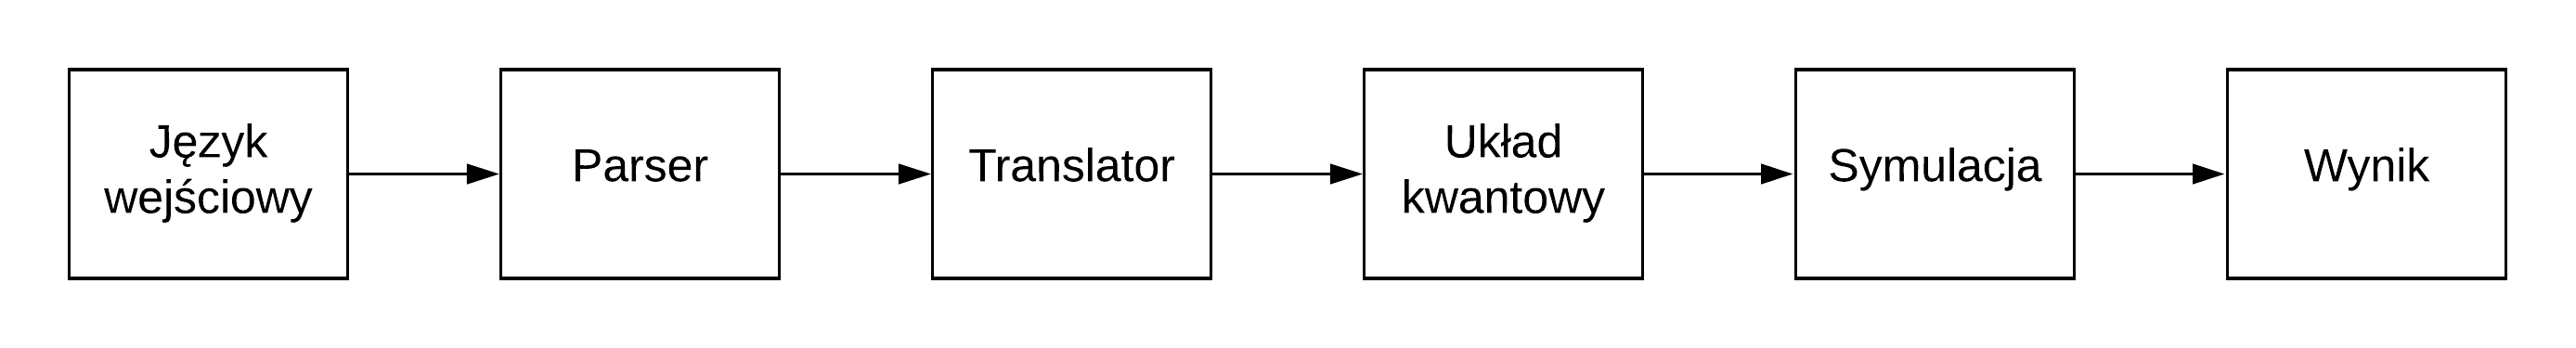
\includegraphics[width=\linewidth]{systemDiag.png}
    \caption{Diagram potoku}
    \label{fig:potok}
\end{figure}
\section{Język wejściowy i Parser}
\subsection{Gramatyka}
\begin{tabular}{ l c l } 
    \textbf{P} & $\rightarrow$ & \textbf{E} \textbf{P} $|$ \textbf{E} \\ 
    \textbf{E} & $\rightarrow$ & var = \textbf{V} $|$ \textbf{Q} \\ 
    \textbf{V} & $\rightarrow$ & var $|$ const $|$ \textbf{K} \\ 
    \textbf{W} & $\rightarrow$ & \textbf{V} , \textbf{W} $|$ \textbf{V} \\
    \textbf{K} & $\rightarrow$ & and( \textbf{W} ) $|$ not( \textbf{V} ) $|$ or( \textbf{W} ) $|$ xor( \textbf{W} )\\
    \textbf{Q} & $\rightarrow$ & hdm( var ) $|$ swp( var , var ) $|$ tfl( \textbf{L} var \textbf{R} ) $|$ \textbf{F}\\
    \textbf{F} & $\rightarrow$ & frd( : var , var , var ) $|$ frd( var , : var , var ) $|$ frd( var , var , : var )\\
    \textbf{L} & $\rightarrow$ & \textbf{L} : var , $|$ $\epsilon$\\
    \textbf{R} & $\rightarrow$ & , : var \textbf{R} $|$ $\epsilon$\\
\end{tabular}
\subsection{Analiza leksykalna}
\begin{center}
    \begin{tabular}{|m{4cm}|m{4cm}|p{7cm}|}
        \hline
        Token & Regex & Opis \\
        \hline
        \texttt{var} & \texttt{[a-zA-Z\_]+} & nazwa zmiennej\\
        \texttt{const} & \texttt{0|1} & stała (możliwe wartości początkowe zmiennej)\\
        \texttt{=} & \texttt{=} & operator przypisania\\
        \texttt{,} & \texttt{,} & separator\\
        \texttt{:} & \texttt{:} & wskaźnik kubitu sterującego\\
        \texttt{and(} ( \texttt{not(}, \texttt{or(}, \texttt{xor(} ) & \texttt{and(} ( \texttt{not(}, \texttt{or(}, \texttt{xor(} ) & otwarcie bramki and (not, or, xor)\\
        \texttt{hdm(} ( \texttt{frd(}, \texttt{swp(}, \texttt{tfl(} ) & \texttt{hdm(} ( \texttt{frd(}, \texttt{swp(}, \texttt{tfl(} ) & otwarcie bramki Hadamarda (Fredkina, SWAP, Toffoliego)\\
        \texttt{)} & \texttt{)} & nawias zamykający \\
        \hline
    \end{tabular}
\end{center}
\subsection{Instrukcje i analiza semantyczna}
\subsubsection{Definiowanie zmiennej poprzez przypisanie jej wartości}
\begin{center}
    \textbf{E} $\rightarrow^*$ var = const
\end{center}
Przypisanie wartości zmiennej jest równe jej deklaracji. Raz zadeklarowanej zmiennej nie można przypisać nowej wartości.
\par Na przykład \texttt{a = 0} jest deklaracją zmiennej o nazwie \texttt{a} z wartością równą 0.
\subsubsection{Obliczenie funkcji boolowskiej na wcześniej zadeklarowanych zmiennych.}
\begin{center}
    \textbf{E} $\rightarrow^*$ var = \textbf{K}
\end{center}
Funkcję boolowską definiuje się poprzez bramki logiczne \texttt{and, or, xor, not}. Bramki \texttt{and, or, xor} są uogólnione do dowolnej liczby zmiennych. Instrukcja ta przypisuje wynik funkcji do zmiennej o nazwie $var$ (leksemu odpowiadającemu temu tokenowi). Zmienna o nazwie $var$ nie może być wcześniej zadeklarowana. Instrukcja ta nie zmienia wartości argumentów funkcji \texttt{and, or, xor, not}. 
\par Na przykład instrukcja \texttt{f = and(a,or(c,not(d)))}, gdzie \texttt{a,b,c} to wcześniej zdefiniowane zmienne, przypisze wartość wyrażenia $\texttt{a} \land (\texttt{c} \lor \neg \texttt{d})$ do zmiennej o nazwie \texttt{f}.
\subsubsection{Operowanie na zdefiniowanych zmiennych przy użyciu wybranych bramek kwantowych.}
\begin{center}
    \textbf{E} $\rightarrow^*$ \textbf{Q}
\end{center}
Bramki kwantowe operują na zadeklarownych zmiennych mutując ich stan. Nie zwracają żadnej wartości.
\par Dla bramek wielokubitowych, które przyjmują zmienne sterujące oraz wejściowe, zmienne sterujące oznaczane są poprzez poprzedzający '\texttt{:}'. Na przykład instrukacja \texttt{tfl(:a, b, :c)} oznacza bramkę Toffoliego na zmiennej wejściowej \texttt{b} ze zmiennymi strującymi \texttt{a}, \texttt{c}.\\
\par Powyższy język umożliwia na konstrukcje opisane w rodziale \ref{rozdzial1}.
\section{Translator}
Opis zagadnienia translacji został wydzielony do rodziału \ref{rozdzial2a}.
\section{Układ kwantowy z rejestrem}
Przez układ kwantowy z rejestrem rozumiemy tutaj parę $(\q, G)$, gdzie $\q$ to stan wejściowy rejestru kubitów, rozumiany jako wektor, a $G$ to ciąg kolejno nakładanych na rejestr bramek. Każda z bramek, na których użycie pozwala omawiany proagram, należy do jednego z poniższych typów:
\begin{itemize}
    \item[\texttt{hdm}] Bramka Hadamarda
    \item[\texttt{tfl}] Uogólniona bramka Toffoliego
    \item[\texttt{frd}] Bramka Fredkina
    \item[\texttt{swp}] Bramka $SWAP$
\end{itemize}
Poza typem, każda bramka zawiera listę parametów. Dla bramki Hadamarda jest to indeks kubitu, w rejestrze kubitu wejściowego. Bramka Toffoliego jest paramatryzowana, poza indeksem kubitu wejściowego (z ang. \textit{target}), przez listę ideksów kubitów sterujących (z ang. \textit{conrol}). Bramka $SWAP$ jest paramatryzowana parą indeków kubitów wejściowych, a bramka Fredkina parą indeków kubitów wejściowych oraz indeksem kubitu sterującego.
\subsection{Przykład}
Następującemu układowi kwantowemu
\[
    \Qcircuit @C=1.5em @R=1.5em {
        \lstick{\ket{0}} & \targ & \ctrl{2} & \qswap & \qw & \rstick{\ket{o_0}} \qw \\
        \lstick{\ket{0}} & \targ & \qw & \qswap & \gate{H} & \rstick{\ket{o_1}} \qw \\
        \lstick{\ket{0}} & \qw & \targ & \ctrl{-2} &\targ & \rstick{\ket{o_2}} \qw \\
        \lstick{\ket{0}} & \qw & \ctrl{-1} & \gate{H} & \qw & \rstick{\ket{o_3}} \qw
    }
\]
odpowiada specyfikacja $(\q, G)$, gdzie
\[\q = \ket{0000}\]
\begin{center}
    $G$ = [ \texttt{not}(0), \texttt{not}(1), \texttt{tfl}([0,3])(2), \texttt{frd}(2)(0,1), \texttt{hdm}(1), \texttt{not}(2) ]
\end{center}
Porządek wykonywania bramek jest nadany od lewej do prawej. Dla bramek znajdujących się w tej samej kolumnie kolejność wykonywania jest nieistotna.
\section{Symulator}
Ciąg sperametryzowanych bramek przekształcana jest na ciąg macierzy odpowiadającym tym bramkom, a następnie przeprowadzana jest operacja mnożenia, która kondensuje listę przekształceń do pojedynczej macierzy $M$. W wyniku opracji monożenia macierzy $M$ przez wektor stanu rejestru otrzymywany jest stan końcowy rejestru. Następnie stan ten jest "mierzony". To znaczy zwracany jest losowo, z prawdopodobieństwem wynikającym ze stanu rejestru, jeden z możliwych do zmierzenia stanów. 
\subsection{Generacja macierzy bramek z ich definicji}
Żeby możliwe było mnożenie macierzy bramki przez stanu rejestru macierz ta musi mieć wymiary $2^n \times 2^n$ dla $n$ kubitowego rejestru. Zatem wszystkie bramki operujące na podzbiorze kubitów z rejestru muszą być rozszerzone tak, by operować na całym rejestrze.
\subsubsection{Bramki jednokubitowe}
\label{oneqgate}
Niech $M$ będzie macierzą bramki operujacej na jednym kubicie. Niech $\q$ będzie rejestrem n kubitów.
Weźmy bramkę o macierzy $M$, która operuje na kubicie o indeksie $i < n$ (kubity numerowane od zera).
\par W celu obliczenia wyniku operacji tej bramki na stanie kwantowym $\q$ należałoby pomnożyć macierz $M$ przez stan kubitu z indeksem $i$. Na stanach pozostałych kubitów należy przeprowadzić operację identyczności (której odpowiada macierz identyczności). Operacja łacząca stany kubitów oraz macierze operacji na pojedynczych kubitach to produkt tensorowy oznaczany $\otimes$.
\par Bramka kwantowa $M$ po rozszerzeniu do n kubitów wygląda następująco:
\[M_n = Id^i \otimes M \otimes Id^{n-i-1}\]
gdzie przez $Id^j$ rozumiemy produkt tensorowy $j$ macierzy identyczności o wymiarach $2 \times 2$.
\subsubsection{Bramki wielokubitowe}
\label{multiqg}
Analogicznie można rozszerzać bramki wielokubitowe jeśli operują na sąsiadujących w rejestrze kubitach.
Jeżeli jednak bity sterujące i/lub bity wejściowe nie sąsiadują to można wykorzystać bramkę $SWAP$ do zamiany kolejności kubitów w rejetrze. Dzięki temu, że każdą permutację można rozbić na złożenie transpozycji, jest to zawsze możliwe do osiągnięcia.
\par Weźmy na przykład układ o rejetrze pięcio-kubitowym z bramką \texttt{tfl([0,3])(2)}. Układ ten został przestawiony na schemacie poniżej po lewej stronie. Diagram po prawej stronie jest równoważny temu układowi, ale wykorzystuje jedynie operacje na sąsiednich kubitach.
\columnratio{0.45, 0.1, 0.45}
\begin{paracol}{3}
    \vspace*{\fill}
    \[
        \Qcircuit @C=1.5em @R=1.5em {
            \lstick{\ket{q_0}} & \qw & \qw & \ctrl{2} & \qw & \qw & \rstick{\ket{q_0'}} \qw \\
            \lstick{\ket{q_1}} & \qw & \qw & \qw & \qw & \qw & \rstick{\ket{q_1'}} \qw \\
            \lstick{\ket{q_2}} & \qw & \qw &\targ & \qw & \qw & \rstick{\ket{q_2'}} \qw \\
            \lstick{\ket{q_3}} & \qw & \qw & \ctrl{-1} & \qw& \qw & \rstick{\ket{q_3'}} \qw \\
            \lstick{\ket{q_4}} & \qw & \qw & \qw & \qw & \qw & \rstick{\ket{q_4'}} \qw
        }
    \]
    \vspace*{\fill}
    \switchcolumn
    \vspace*{\fill}
    \centering
    =
    \vspace*{\fill}
    \switchcolumn
    \vspace*{\fill}
    \[
        \Qcircuit @C=1.5em @R=1.5em {
            \lstick{\ket{q_0}} & \qswap & \qw & \qw & \qw & \qswap & \rstick{\ket{q_0'}} \qw \\
            \lstick{\ket{q_1}} & \qswap \qwx & \qw & \ctrl{1} & \qw & \qswap \qwx & \rstick{\ket{q_1'}} \qw \\
            \lstick{\ket{q_2}} & \qw & \qswap &\ctrl{1} & \qswap & \qw & \rstick{\ket{q_2'}} \qw \\
            \lstick{\ket{q_3}} & \qw & \qswap \qwx & \targ & \qswap \qwx & \qw & \rstick{\ket{q_3'}} \qw \\
            \lstick{\ket{q_4}} & \qw & \qw & \qw & \qw & \qw & \rstick{\ket{q_4'}} \qw
        }
    \]  
    \vspace*{\fill}
\end{paracol}
Zatem można rozpisać $\texttt{tfl([0,3])(2)} = \texttt{swp(0,1)} * \texttt{swp(2,3)} * \texttt{tfl([0,3])(2)} * \texttt{swp(0,1)} * \texttt{swp(2,3)}$. Wtedy jeśli każda z wykorzystwanych bramek zostanie rozszerzona, tak by operowała na pięciu kubitach, zgodnie ze strategią opisaną z rodziale \ref{oneqgate}, to zostanie wygenerowana macierz wykonująca operację \texttt{tfl([0,3])(2)} na rejestrze piecio-kubitowym.
% Wtedy otrzymujemy poniższą macierz (zera zastąpione pustymi miejscami dla czytelności).
% \setcounter{MaxMatrixCols}{35}
% \[
%     \begin{bmatrix}
%         1 &   &   &   &   &   &   &   &   &   &   &   &   &   &   &   &   &   &   &   &   &   &   &   &   &   &   &   &   &   &   &  \\
%           & 1 &   &   &   &   &   &   &   &   &   &   &   &   &   &   &   &   &   &   &   &   &   &   &   &   &   &   &   &   &   &  \\
%           &   & 1 &   &   &   &   &   &   &   &   &   &   &   &   &   &   &   &   &   &   &   &   &   &   &   &   &   &   &   &   &  \\
%           &   &   & 1 &   &   &   &   &   &   &   &   &   &   &   &   &   &   &   &   &   &   &   &   &   &   &   &   &   &   &   &  \\
%           &   &   &   & 1 &   &   &   &   &   &   &   &   &   &   &   &   &   &   &   &   &   &   &   &   &   &   &   &   &   &   &  \\
%           &   &   &   &   & 1 &   &   &   &   &   &   &   &   &   &   &   &   &   &   &   &   &   &   &   &   &   &   &   &   &   &  \\
%           &   &   &   &   &   & 1 &   &   &   &   &   &   &   &   &   &   &   &   &   &   &   &   &   &   &   &   &   &   &   &   &  \\
%           &   &   &   &   &   &   & 1 &   &   &   &   &   &   &   &   &   &   &   &   &   &   &   &   &   &   &   &   &   &   &   &  \\
%           &   &   &   &   &   &   &   & 1 &   &   &   &   &   &   &   &   &   &   &   &   &   &   &   &   &   &   &   &   &   &   &  \\
%           &   &   &   &   &   &   &   &   & 1 &   &   &   &   &   &   &   &   &   &   &   &   &   &   &   &   &   &   &   &   &   &  \\
%           &   &   &   &   &   &   &   &   &   & 1 &   &   &   &   &   &   &   &   &   &   &   &   &   &   &   &   &   &   &   &   &  \\
%           &   &   &   &   &   &   &   &   &   &   & 1 &   &   &   &   &   &   &   &   &   &   &   &   &   &   &   &   &   &   &   &  \\
%           &   &   &   &   &   &   &   &   &   &   &   & 1 &   &   &   &   &   &   &   &   &   &   &   &   &   &   &   &   &   &   &  \\
%           &   &   &   &   &   &   &   &   &   &   &   &   & 1 &   &   &   &   &   &   &   &   &   &   &   &   &   &   &   &   &   &  \\
%           &   &   &   &   &   &   &   &   &   &   &   &   &   & 1 &   &   &   &   &   &   &   &   &   &   &   &   &   &   &   &   &  \\
%           &   &   &   &   &   &   &   &   &   &   &   &   &   &   & 1 &   &   &   &   &   &   &   &   &   &   &   &   &   &   &   &  \\
%           &   &   &   &   &   &   &   &   &   &   &   &   &   &   &   & 1 &   &   &   &   &   &   &   &   &   &   &   &   &   &   &  \\
%           &   &   &   &   &   &   &   &   &   &   &   &   &   &   &   &   & 1 &   &   &   &   &   &   &   &   &   &   &   &   &   &  \\
%           &   &   &   &   &   &   &   &   &   &   &   &   &   &   &   &   &   &   &   &   &   & 1 &   &   &   &   &   &   &   &   &  \\
%           &   &   &   &   &   &   &   &   &   &   &   &   &   &   &   &   &   &   &   &   &   &   & 1 &   &   &   &   &   &   &   &  \\
%           &   &   &   &   &   &   &   &   &   &   &   &   &   &   &   &   &   &   &   & 1 &   &   &   &   &   &   &   &   &   &   &  \\
%           &   &   &   &   &   &   &   &   &   &   &   &   &   &   &   &   &   &   &   &   & 1 &   &   &   &   &   &   &   &   &   &  \\
%           &   &   &   &   &   &   &   &   &   &   &   &   &   &   &   &   &   & 1 &   &   &   &   &   &   &   &   &   &   &   &   &  \\
%           &   &   &   &   &   &   &   &   &   &   &   &   &   &   &   &   &   &   & 1 &   &   &   &   &   &   &   &   &   &   &   &  \\
%           &   &   &   &   &   &   &   &   &   &   &   &   &   &   &   &   &   &   &   &   &   &   &   & 1 &   &   &   &   &   &   &  \\
%           &   &   &   &   &   &   &   &   &   &   &   &   &   &   &   &   &   &   &   &   &   &   &   &   & 1 &   &   &   &   &   &  \\
%           &   &   &   &   &   &   &   &   &   &   &   &   &   &   &   &   &   &   &   &   &   &   &   &   &   &   &   &   &   & 1 &  \\
%           &   &   &   &   &   &   &   &   &   &   &   &   &   &   &   &   &   &   &   &   &   &   &   &   &   &   &   &   &   &   & 1\\
%           &   &   &   &   &   &   &   &   &   &   &   &   &   &   &   &   &   &   &   &   &   &   &   &   &   &   &   & 1 &   &   &  \\
%           &   &   &   &   &   &   &   &   &   &   &   &   &   &   &   &   &   &   &   &   &   &   &   &   &   &   &   &   & 1 &   &  \\
%           &   &   &   &   &   &   &   &   &   &   &   &   &   &   &   &   &   &   &   &   &   &   &   &   &   & 1 &   &   &   &   &  \\
%           &   &   &   &   &   &   &   &   &   &   &   &   &   &   &   &   &   &   &   &   &   &   &   &   &   &   & 1 &   &   &   &  \\
%     \end{bmatrix} 
% \]
\subsubsection{Uogólniona bramka Toffoliego}
Uogólniona bramka Toffoliego wykonuje operację negacji na bicie wejściowym gdy wszystkie bity strerujące są jedynkami.
\par Opisana w rodziale \ref{multiqg} bramka \texttt{tfl([0,3])(2)} operująca na pięcio-kubitowym rejestrze mapuje czyste stany kwantowe następująco:
\[10010  \rightarrow 10110\;\text{ i }\;10110  \rightarrow 10010\] %18 - 22
\[11010  \rightarrow 11110\;\text{ i }\;11010  \rightarrow 11110\] %26 - 30
\[10011  \rightarrow 10111\;\text{ i }\;10011  \rightarrow 10111\] %19 -23
\[11011  \rightarrow 11111\;\text{ i }\;11011  \rightarrow 11111\] %27 - 31
w pozostałych przypadkach dokonuje mapowania identycznościowego.
\par Bramka Toffoliego jest macierzą permutacji, która w każdym wierszu oraz kolumnie ma dokładnie jedną jedynką oraz $n-1$ zer. Dla mapowania
\[10010  \rightarrow 10110\]
jedynka powinna się znaleźć w 19 kolumnie, 23 wierszu, ponieważ 
\[10010_{(2)} = 18\]
\[10110_{(2)} = 22\]
gdzie numaracja zaczyna się od zera.\\
\begin{pseudokod}[H]
    \SetArgSty{normalfont}
    \KwIn{Liczba kubitów w rejestrze $n$, zbiór indeksów bitów sterujących $C$, indeks bitu wejściowego $i$}
    \KwOut{Macierz bramki Toffoliego M}
    $M \leftarrow$ macierz wymiarów $2^n \times 2^n$ wypełniona 0\\
    \For{$j \leftarrow 0$ \KwTo $2^n$}{
        $isId \leftarrow$ \texttt{false}\\
        \ForEach{$c \in C$}{
            \tcc{bity w zapisie biranym numerujemy od najmiej znaczącego, indeksem 0}
            \If{$j$ ma 0 na ($n-c-1$)-tym bicie w zapisie binarnym}{
                $isId \leftarrow$ \texttt{true}
            }
        }
        \If{$idId$}{
            \tcc{przypadek gdy, wszystkie kubity sterujące są jedynkami}
                wstaw 1 do macierzy M na miejscu ($j$, $j$ bitwise\_not na ($n-i$)-tym bicie) \tcc{(kolumna, wiersz)}
        }
        \Else {
                wstaw 1 do macierzy M na miejscu ($j$, $j$)
        }
    }
    \caption{Generacja macierzy bramki Toffoliego z defninicji bramki}\label{alg:toffoliGateGen}
\end{pseudokod}
\section{Wyjście}
Program zwraca schemat układu kwantowego, który został stworzony w wyniku działania translatora. Układ ten odpowiada obliczeniom zdefiniowanym w opisie wejściowym.
\par Poza układem program zwraca wynik obliczeń, czyli końcowy, zmierzony, stan rejestru kwantowego po symulacji działania układu kwantowego. Dodatkowo zwaraca informację o prawdopodobienstwie otrzymania stanu $\ket{1}$ dla każdego z kubitów w rejestrze.
	\cleardoublepage

	\chapter{Translacja układów logicznych do układów kwantowych}
\thispagestyle{chapterBeginStyle}
\label{rozdzial2a}
Jednym z najważniejszych zagadnień, którymi zajmuje się ta praca, jest translacja układów logicznych, rozumianych jako zestaw funkcji boolowskich (rodział \ref{rozdzial0a}), do układów kwantowych. Celem przedstawionego tu problemu translacji jest stworzenie układu kwantowego, który oblicza te same funkcje boolowskie co zadany układ, z wykorzystaniem zestawu bramek przedstawionego we wcześniejszych rozdziałach, czyli bramek należących do rodziny bramek Toffoliego, bramki $SWAP$ oraz bramki Fredkina. 
\section{Problem translacji}
W przeciwieństwie do bramek logicznych, operacje składające się na układ kwantowy muszą być unitarne. W szczególności znaczy to, że przyjmują na wejściu tyle samo bitów ile zwracają na wyjściu. Zatem chcąc wyrazić te same operacje, które wykonuje układ logiczny za pomocą układu kwantowego, traktowanego tutaj jako pojedyncza operacja, należałoby odpowiednio zwiększyć liczbę bitów na wejściu/wyjściu i następnie zignorować te ,,dodatkowe'' bity na wejściu/wyjściu. Nie zapewnia to jednak, że tak stworzone mapowanie przedstawione jako macierz będzie poprawną bramką kwantową (tzn. czy macierz ta będzie unitarna).
\par Weźmy na przykład układ logiczny składający się z pojedynczej bramki $AND$. Żeby zachować stałą liczbę bitów na wejściu i wyjściu możemy stworzyć funkcję:
\[f_{AND}(a,b) = (0, ab)\]
Tak stworzona fukcja nie jest nawet odwracalna, co jest warunkiem koniecznym unitarności. Co więcej, nie istnieje taka funckcja boolowska $h$
\[f_{AND}(a,b) = (h(a,b), ab)\]
żeby $f_{AND}$ było funkcją odwracalną.
\par Dlatego symulowanie układów logicznych za pomocą układów kwantowych wymaga czasami wprowadzenia bitów pomocniczych, które stanowią dodatkową przestrzeń do obliczeń i których wartość początkowa jest znana, tutaj zawsze $\ket{0}$.
\section{Podejście naiwne}
\label{naive}
Jeżeli stworzony układ kwantowy nie jest pojedynczą bramką, a ciągiem operacji, to każda z tych operacji musi być unitarna. Oznacza to w szczególności, że nie tylko liczby bitów na wejściu do układu i wyjściu z układu muszą być sobie równe, ale że liczba bitów, na których bramki kwantowe operują jest stała. W szczególności nie można dokonać ,,rodzielenia kabla'' jak to się dzieje w przypadku układów klasycznych.
\par Dlatego o każdej takiej opracji będziemy myśleć jako o bramce $COPY$, której zachowanie można zapisać za pomocą funkcji następująco:
\[COPY(a) = (a,a)\] 
\par Jeżeli potrafimy wyrazić bramkę $COPY$ oraz zestaw bramek logicznych tworzących układ funkcjonalnie zupełny za pomocą bramek kwantowych, to potrafimy wyrazić każdy układ logiczny za pomocą układu kwantowego.
\par Zatem naturalnie pierwszym podejściem do problemu translacji układów logicznych na kwantowe jest wyrażenie tego układu używając jedynie pewnego ograniczonego (zupełnego) zestawu bramek, na przykład $COPY, NOT, AND$, a następnie bezpośrednia zamiana każdej z tych operacji na bramki kwantowe.
\subsection{Copy}
Ze względu na stałą liczbę kubitów w układzie kwantowym, każda bramka $COPY$ wymaga powiększenia rejestru wejściowego o jeden bit. Zatem kwantowa bramka $COPY$ będzie dokonywała mapowania 
\[C(a,0) = (a,a)\]
dla $a \in \{0,1\}$.
\par Operację tę można wyrazić za pomocą bramki Feymana
\[
    \Qcircuit @C=1.5em @R=1.5em {
        \lstick{\ket{a}} & \ctrl{1} & \rstick{\ket{a}} \qw \\
        \lstick{\ket{0}} & \targ & \rstick{\ket{0 \otimes a} = \ket{a}} \qw
    }
\]
\subsection{Not}
Logicznej operacji Not odpowiada bramka kwantowa $NOT$.
\subsection{And}
Weźmy funkcję
\[T(a,b,c) = (a,b, c \otimes ab)\]
Wtedy jeżeli $c = 0$ to
\[T(a,b,0) = (a,b, ab)\]
Operacji tej odpowiada bramka Toffoliego:
\[
    \Qcircuit @C=1.5em @R=1.5em {
        \lstick{\ket{a}} & \ctrl{1} & \rstick{\ket{a}} \qw \\
        \lstick{\ket{b}} & \ctrl{1} & \rstick{\ket{b}} \qw \\
        \lstick{\ket{0}} & \targ & \rstick{\ket{0 \otimes ab} = \ket{ab}} \qw
    }
\]
Zatem po wprowadzeniu bitu pomocniczego można obliczyć And za pomocą bramki Toffoliego.
\section{Wyrażanie funkcji boolowskich za pomocą układów kwantowych}
\subsection{Wejście}
W niniejszej pracy, zgodnie z modelem przedstawionym w rozdziale \ref{rozdzial0a}, myślimy jako o wektorze funkcji boolowskich. Zatem wejściem do translatora jest funkcja boolowska, ponieważ będzimy zajmować się ,,jedną na raz''. Dodatkowo zakładamy, że każda zadeklarowana zmienna jest również częścią wyjścia, zatem nie możemy ,,utracić'' wartości tych zmiennych.
\subsection{Przykład}
Weźmy przykładową funkcję
\[f(a,b,c) = b + a\overline{c} = b \lor (a \land (\neg c))\]
Korzystając z metod translacji opisanych w rozdziale \ref{naive}, można przestawić tę funkcję w następujący sposób:
\[
    \Qcircuit @C=1.5em @R=1.5em {
        \lstick{\ket{a}} & \qw & \ctrl{2} & \qw & \qw & \qw & \qw & \rstick{\ket{a}} \qw \\
        \lstick{\ket{b}} & \qw & \qw & \qw & \targ & \ctrl{2} & \targ & \rstick{\ket{b}} \qw \\
        \lstick{\ket{c}} & \targ & \ctrl{1} & \targ & \qw & \qw & \qw & \rstick{\ket{c}} \qw \\
        \lstick{\ket{0}} & \qw & \targ & \qw & \targ & \ctrl{1} & \targ & \rstick{\ket{a\overline{c}}} \qw \\
        \lstick{\ket{0}} & \qw & \qw & \qw & \qw & \targ & \targ & \rstick{\ket{b + a\overline{c}}} \qw
    }
\]
Na wejściu zostały dodane dwa bity. Używając strategii tłumaczenia każdej operacji $AND, OR, NOT$ na zestaw bramek kwantowych liczba potrzebnych kubitów pomocniczych rośnie z sumaryczną liczbą bramek $OR$ i $AND$. Jeden bit na wejściu jest konieczny to przechowania wyniku funkcji, ale wartości przechowywane na reszcie z kubitów pomocniczych są niestotne.
\subsection{Teoretyczne minimum dla bitów pomocniczych}
\begin{lemma}
    \label{l:min}
    Z każdej funkcji boolowskiej $f(\vec{x}) = f(x_0, x_1, \ldots x_n)$, dla pewnego $n \in \mathbb{N}$ oraz $\vec{x} \in \{0, 1\}^n$, można stworzyć funkcję $f_Q : \{0, 1\}^{n+1}\rightarrow \{0, 1\}^{n+1}$, dla której 
    \[f_Q(x_0, x_1, \ldots x_n, 0) = (x_0, x_1, \ldots x_n, f(x_0, x_1, \ldots x_n))\] 
    oraz, której odpowiada macierz unitarna wymiarów $2^{n+1} \times 2^{n+1}$.
\end{lemma}
\begin{proof}
    Zdefiniujmy $f_Q$ następująco
    \[f_Q(x_0, x_1, \ldots x_n, c) = (x_0, x_1, \ldots x_n, c \otimes f(\vec{x}))\]
    Wtedy dla c = 0
    \[f_Q(x_0, x_1, \ldots x_n, 0) = (x_0, x_1, \ldots x_n, 0 \otimes f(\vec{x}))\]
    Funkcją przeciwną do $f_Q$ jest ona sama.
    \[f_Q(f_Q(x_0, x_1, \ldots x_n, c)) = (x_0, x_1, \ldots x_n, c \otimes f(\vec{x}) \otimes f(\vec{x})) = (x_0, x_1, \ldots x_n, c)\]
    Ponieważ funkcja $f_Q$ jest bijekcją, można wyrazić ją jako permutację na wektorach $\{0,1\}^{n+1}$. Dla macierzy $M$ wyrażającej tę permutację otrzymujemy $\forall x_0, x_1, \ldots x_n \in \{0,1\}^{n+1}$
    \[MM\ket{x_0, x_1, \ldots x_n} = \ket{x_0, x_1, \ldots x_n}\]
    Stąd
    \[MM = I\]
\end{proof}
Z lematu \ref{l:min} wynika, że każdą funkcję boolowską można można wyrazić za pomocą układu kwantowego z użyciem tylko jednego bitu pomocniczego, który na wyjściu przechowuje wynik tej funkcji.
\section{Postać ESOP}
W rozdziale \ref{rozdzial0a} omówiona została sumacyjna postać kanoniczna fukcji boolowskiej. Funkcja w tej postaci jest wyrażona jako suma produktów (termów). Analogiczną postacią jest postać ESOP czyli alternatywa wykluczająca termów.
\begin{theorem}
    Każdą funkcję boolowską można zapisać w postaci ESOP.
\end{theorem}
\begin{proof}
    Weźmy funkcję boolowską $f: \{0, 1\}^n \rightarrow \{0, 1\}$ zapisaną w postaci sumy mintermów.
    \[f(a_0, a_1, \ldots a_n) = m_{k_0} + m_{k_1} + \ldots + m_{k_l}\]
    gdzie $m_i$ oznacza minterm, a $k_0, k_1, k_l \in \{0, 1, \ldots n\}$ oznaczają indeksy mintermów należących do funkcji f.\\
    Zauważmy następującą tożsamość
    \[a + b = a \otimes b \otimes ab\]
    Wtedy, ponieważ $\forall i,j$
    \[m_i \otimes m_j = 0\]
    funkcję $f$ można zapisać
    \[f(a_0, a_1, \ldots a_n) = m_{k_0} \otimes m_{k_1} \otimes \ldots \otimes m_{k_l}\]
\end{proof}
\section{Tworzenie układu kwantowego z postaci ESOP}
\begin{theorem}
    Każdą funkcję boolowską $f: \{0, 1\}^n \rightarrow \{0,1\}$ można obliczyć za pomocą układu o rejestrze ($n+1$)-kubitowym, składającego się z maksymalnie $2^n$ uogólnionych bramek Toffoliego oraz $2^{n+1}*n$ bramek $NOT$.
\end{theorem}
\begin{proof}
    Weźmy funkcję $f$ w postaci alternatywy wykluczającej mintermów.
    \[f(a_0, a_1, \ldots a_n) = m_{k_0} \otimes m_{k_1} \otimes \ldots \otimes m_{k_l}\]
    Wtedy każdy minterm można obliczyć za pomocą maksymalnie $n*2$ bramek $NOT$ oraz uogólnionej bramki Toffoliego rozmiaru $n+1$. Pierwsze maksymalnie $n$ bramek $NOT$ jest używanych do otrzymania wartości literałów tworzących mineterm. Następnie bramka Toffoliego jest wykorzytana do obliczenia wartościowania mintermu i zapisania go na bicie pomocniczym. Pozostałe bramki $NOT$ są wykorzystane do przywrócenia stanów wejściowych na bitach argumentów.
    \par Dla przykładowego mintermu $m = x_0x_1\overline{x_2}\overline{x_3}x_4$ konstrukacja ta wygląda następująco:
    \columnratio{0.45, 0.1, 0.45}
    \begin{paracol}{3}
        \vspace*{\fill}
    \[
        \Qcircuit @C=1.5em @R=1.5em {
            \lstick{\ket{x_0}} & \qw & \ctrl{1} & \qw & \rstick{\ket{x_0}} \qw \\
            \lstick{\ket{x_1}} & \qw & \ctrl{1} & \qw & \rstick{\ket{x_1}} \qw \\
            \lstick{\ket{x_2}} & \qw & \ctrl{1} & \qw & \rstick{\ket{x_2}} \qw \\
            \lstick{\ket{x_3}} & \qw & \ctrl{1} & \qw & \rstick{\ket{x_3}} \qw \\
            \lstick{\ket{x_4}} & \qw & \ctrl{1} & \qw & \rstick{\ket{x_4}} \qw \\
            \lstick{\ket{0}} & \qw & \gate{m_i} & \qw & \rstick{\ket{m}} \qw
        }
    \]
    \vspace*{\fill}
    \switchcolumn
    \vspace*{\fill}
    \begin{center}
        =
    \end{center}
    \vspace*{\fill}
    \switchcolumn
    \vspace*{\fill}
    \[
        \Qcircuit @C=1.5em @R=1.5em {
            \lstick{\ket{x_0}} & \qw & \ctrl{1} & \qw & \rstick{\ket{x_0}} \qw \\
            \lstick{\ket{x_1}} & \qw & \ctrl{1} & \qw & \rstick{\ket{x_1}} \qw \\
            \lstick{\ket{x_2}} & \targ & \ctrl{1} & \targ & \rstick{\ket{x_2}} \qw \\
            \lstick{\ket{x_3}} & \targ & \ctrl{1} & \targ & \rstick{\ket{x_3}} \qw \\
            \lstick{\ket{x_4}} & \qw & \ctrl{1} & \qw & \rstick{\ket{x_4}} \qw \\
            \lstick{\ket{0}} & \qw & \targ & \qw & \rstick{\ket{m}} \qw
        }
    \]
    \vspace*{\fill}
    \end{paracol}
    \par Korzystając z tak zbudowanych framgentów układu obliczających wartości mintermów można stworzyć następujący układ kwantowy.
        \[
            \Qcircuit @C=1.5em @R=1.5em {
                & \lstick{\ket{x_0}} & \ctrl{1} & \ctrl{1} & \qw & \ldots & & \ctrl{1} & \rstick{\ket{x_0}} \qw \\
                & \lstick{\ket{x_1}} & \ctrl{1} & \ctrl{1} & \qw & \ldots & & \ctrl{1} & \rstick{\ket{x_1}} \qw \\
                \vdots & & \vdots & \vdots & & \ddots & & \vdots & & \vdots & \\
                & \lstick{\ket{x_n}} & \ctrl{1} & \ctrl{1} & \qw & \ldots & & \ctrl{1} & \rstick{\ket{x_n}} \qw \\
                & \lstick{\ket{0}} & \gate{m_{k_0}} & \gate{m_{k_1}} & \qw & \ldots & & \gate{m_{k_l}} & \rstick{\ket{((\ldots((0 \otimes m_{k_0}) \otimes m_{k_1}) \ldots )\otimes m_{k_l})}} \qw
            }
        \]
    Ostatni bit powyższego układu ,,zbiera'' wartości mintermów. Jeśli na wejsciu był on zerem to na wyjściu będzie przechowywał wartość funkcji $f$.
\end{proof}
\subsection{Przykład}
Weźmy przykładową funkcję
\[f(a,b,c,d) = ab \otimes \overline{a}\overline{b}cd \otimes \overline{a}\overline{c}\]
w postaci alternatywy wykluczającej termów.
\par Wtedy układ kwantowy, zbudowany z bramek $NOT$ oraz bramek Toffoliego, wyrażający tę funkcję, wygląda następująco:
\[
    \Qcircuit @C=1.5em @R=1.5em {
        \lstick{\ket{a}} & \ctrl{1} & \targ & \ctrl{1} & \targ & \targ &  \ctrl{2} & \targ & \rstick{\ket{a}} \qw \\
        \lstick{\ket{b}} & \ctrl{3} & \targ & \ctrl{1} & \targ & \qw &    \qw &      \qw & \rstick{\ket{b}} \qw \\
        \lstick{\ket{c}} & \qw &      \qw &   \ctrl{1} & \qw &   \targ &  \ctrl{2} & \targ & \rstick{\ket{c}} \qw \\
        \lstick{\ket{d}} & \qw &      \qw &   \ctrl{1} & \qw &   \qw &    \qw &       \qw & \rstick{\ket{d}} \qw \\
        \lstick{\ket{0}} & \targ &    \qw &   \targ &    \qw &   \qw &    \targ &     \qw & \rstick{\ket{f}} \qw 
    }
\]
\subsection{Algorytm}
W celu optymalizacji bramek $NOT$ wykorzystanych w układzie obliczającym funkcję $f$ algorytm przetrzymuje informację o aktualnym stanie zmiennych, to znaczy informację, czy kubit odpowiadający danej zmiennej przechowuje jej wartość czy negację tej wartości. Dzięki temu wartości argumentów nie są przywracane po każdej bramce Toffoliego, ale jedynie raz na sam koniec.\vspace{4mm}\\
\begin{pseudokod}[H]
    \SetArgSty{normalfont}
    \KwIn{Zbiór termów funkcji w postaci ESOP $E$, index wyjścia $o$}
    \KwOut{Lista bramek kwantowych $G$}
    $negPol \leftarrow$ pusta lista \tcp*{zbiór aktualnie zagenowanych zmiennych}
    $G \leftarrow$ pusta lista \;
    \ForEach{$t \in E$}{
        \ForEach{$v \in t$} { 
            \If {$v$ postaci $\overline{x}$, gdzie x to zmienna}{
                \If { $v.id \notin negPol$} {
                    do $G$ dodaj \texttt{not}($v.id$) \;
                    do $negPol$ dodaj $v.id$ \;
                }
            } \Else {
                \If { $v.id \in negPol$} {
                    do $G$ dodaj \texttt{not}($v.id$) \;
                    z $negPol$ usuń $v.id$ \;
                }
            }
        }
        do $G$ dodaj \texttt{tfl}(lista $id$ elementów z $t$)($o$) \;
    }
    \tcc{przywrócenie stanu początkowego}
    \ForEach{$i \in negPol$}{ 
        do $G$ dodaj \texttt{not}($i.id$) \;
    }
    \caption{Konwersja postaci ESOP to listy bramek kwantowych}\label{alg:esop}
\end{pseudokod}
\section{Rozwinięcie Shannona}
Wejściem do tranlatora są funkcje boolowskie zdefiniowane za pomocą bramek logicznych $AND$, $NOT$, $OR$ oraz $XOR$. Zatem, że przekształcić każdą z tych funkcji na serię bramek kwantowych muszą być najpierw przekształcone do postaci alternatywy wykluczającej termów. Najprostszym podejściem mogłoby być wyliczenie całej tabeli funkcji i przedstawienie jej jako alternatywa wykluczająca mintermów.
\par Weźmy następująco zdefiniowaną funkcję
\[f(\vec{x}) = and(x_0, h(\vec{x}))\]
gdzie $\vec{x}$ jest wektorem długości $n \in \mathbb{N}$, a $h$ funkcją stała równą 1.\\
Do wyrażenia tej funkcji potrzeba $\frac{1}{2}n$ mintermów, które zostaną zamienione na $\frac{1}{2}n$ bramek Toffoliego. Jest to wysoko nieoptymalne, kiedy do obliczenia tej funkcji wystarczy jedna bramka Feymana.
\[
    \Qcircuit @C=1.5em @R=1.5em {
        & \lstick{\ket{x_0}} & \ctrl{4} & \rstick{\ket{a}} \qw & \\
        & \lstick{\ket{x_1}} & \qw & \rstick{\ket{a}} \qw & \\
        \vdots & \vdots & & \vdots & \vdots \\
        & \lstick{\ket{x_n}} & \qw & \rstick{\ket{a}} \qw & \\
        & \lstick{\ket{0}} & \targ & \rstick{\ket{f(\vec{x})}} \qw &
    }
\]
Zamiast wyliczać całą tabelę wartościowań dla funkcji boolowskiej, można zbudować drzewo decyzyjne. 
\begin{definition}
    Rozwinięcie Shannona dla funkcji boolowskiej $f$ względem zmiennej $x_i$ denifiuje się następująco
    \[f(x_0, x_1, \ldots x_n) = x_i*f_{x_i} \otimes \overline{x_i}*f_{\overline{x_i}}\]
    gdzie 
    \[f_{x_i} = f(x_i = 1)\]
    \[f_{\overline{x_i}} = f(x_i = 0)\]
    To znaczy, $f_{x_i}$ jest funkcją powstałą przez podstawienie za $x_i$ $1$.
\end{definition}
\subsection{Algorytm}
\par Korzystając z rozwinięć Shannona budujemy drzewo w następujący sposób:
\begin{enumerate}
    \item Podstaw pod korzeń funkcję $f$. Niech $f' := f$.
    \item Jeśli $f'$ nie jest funkcją stałą przejdź do kolejnego kroku, w przeciwnym przypadku koniec.
    \item Niech $a$ będzie dowolnym z argumentów funkcji $f'$.
    \item Podstaw jako prawego syna węzła z $f'$ $f'_{a}$, jako lewego $f'_{\overline{a}}$.
    \item Wykonaj kroki od 2. dla synów $f'$.
\end{enumerate}
Algorytm ten zwraca drzewo kolejnych rozwinięć o następującej strukturze:
\begin{center}
    \Tree[.$f$ 
        [.$f_{x_0}$ 
            [.$f_{x_0, x_1}$ [.{\vdots} ] [.{\vdots} ]] 
            [.$f_{x_0, \overline{x_1}}$ [.{\vdots} ] [.{\vdots} ]]
        ] 
        [.$f_{\overline{x_0}}$ 
            [.$f_{\overline{x_0}, x_1}$ [.{\vdots} ] [.{\vdots} ]]
            [.$f_{\overline{x_0}, \overline{x_1}}$ [.{\vdots} ] [.{\vdots} ]]
        ]
    ]   
\end{center}
Korzystając z tak zdubowanego drzewa można łatwo znaleźć postać alternatywy wykluczającej termów funkcji $f$. Każdy liść zawiera funkcję stałą, której odpowiada term. Na przykład dla liścia $f_{x_0, \overline{x_1}, x_2}$ mamy term $x_0\overline{x_1}x_2$. Wartość tej funkcji jest wskaźnikiem czy dany term należy do funkcji $f$.
\subsubsection{Przykład} 
Dla przykładowej funkcji $f(a,b,c) = a \land (b \lor \neg c)$ algorytm stworzy następujące drzewo:
\begin{center}
    \Tree[.$f$ 
        [.{$f_{a} = b \lor \neg c$} 
            [.{$f_{a, b} = 1$} ] 
            [.{$f_{a, \overline{b}} = \neg c$}
                [.{$f_{a, \overline{b}, c} = 0$} ]
                [.{$f_{a, \overline{b}, \overline{c}} = 1$} ]
            ] 
        ] 
        [.{$f_{\overline{a}} = 0$} ]
    ]   
\end{center}
Stąd 
\[f(a, b, c) = ab \otimes a\overline{b}\overline{c}\]
	\cleardoublepage
	
	\chapter{Implementacja systemu}
\thispagestyle{chapterBeginStyle}
\label{rozdzial3}

\section{Opis technologii}
Do napisania programu został wykorzystany język Scala w wersji 2.12.8. Do operacji na macierzach została wykorzystana bibiolteka Breeze \footnote{\url{https://github.com/scalanlp/breeze}}. Do napisania parsera została wykorzystana natywna biblioteka Scali, scala-parser-combinators.
\footnote{\url{https://github.com/scala/scala-parser-combinators}}.
\section{Instrukcja obsługi}
Warunkiem wstępnym do skorzystania z programu jest posiadanie zainstalowanego Java JDK w wersji 8 lub wyższej. Program przyjmuje na wejściu jeden lub dwa argumenty. Pierwszym jest ścieżka do pliku zawierającego instrukcje napisane przy użyciu języka opisanego w rozdziale \ref{rozdzial2}. Drugim argumentem jest ścieżka do pliku, do którego ma zostać zapisane rozwiązanie. W przypadku bramku drugiego argumentu rozwiązanie zostanie wypisane bezpośrednio na konsolę.
\section{Język wyjścia}
\begin{verbatim}
a  <1>  -H- --- -●- -x- -○- -x- <0>  0.0
b  <0>  --- --- --- --- --- --- <0>  0.0
c  <0>  --- --- -●- -●- --- -x- <1>  0.5
d  <1>  --- -H- -○- -x- --- --- <0>  0.5
\end{verbatim}
W pierwszej kolumnie widać nazwy zmiennych, które odpowiadają kubitom. Następna kolumna zawiera wartości początkowe. 
\par Dalej jest widoczny układ kwantowy. '\texttt{H}' to bramka Hadamarda, bramka Toffoliego oznaczona jest przez '○' dla bitu wejściowego i '●' dla bitów sterujących, w szeczólności w piątej kolumnie powyższego układu widać bramkę NOT. Bramka Fredkina analogicznie wykorzystuje oznaczenie '●' dla bitów strerujących oraz, tak samo jak bramka SWAP, '\texttt{x}' dla bitów wejściowych.
\par Po schemacie układu kwantowego są wartości wynikowe dla każdego z kubitów, czyli stany kubitów po zmierzeniu ich wartości oraz na końcu prawdobodobieństwo zmierzenia stanu $\ket{1}$ dla każdego z kubitów w rejestrze.
	\cleardoublepage

	\chapter{Przykłady użycia}
\thispagestyle{chapterBeginStyle}
\label{rozdzial4}
	\cleardoublepage
	
	\chapter{Podsumowanie}
\thispagestyle{chapterBeginStyle}
W pracy udało się spełnić wszystkie pierwotne wymagania. W jej wyniku został stworzony program, który pozwala na zamodelowanie na wejściu układu logicznego i tworzy odpowiadający mu układ kwantowy. Program symuluje również działanie układu kwantowego dla pewnego podzbioru bramek kwantowych.
\section{Minimalizacja liczby kubitów pomocniczych}
Głównym zainteresowaniem optymalizacyjnym w tej pracy było generowanie układów kwantowych w sposób, który minimalizuje używane kubity pomocnicze. Program w tym celu wykorzystuje algorytm oparty o uzykanie postaci ESOP dla funkcji boolowskich, a następnie zamianę tej postaci na ciąg bramek z rodziny Toffoliego oraz bramek $NOT$. W wyniku zastosowania tej metody wykorzystywany jest jedynie jeden kubit pomocniczy dla każdej wyjściowej funkcji boolowskiej. Na wyjściu ten kubit przechowuje wartość tej funkcji.
\subsection{Wnioski i uwagi}
Podczas przeprowadzania obliczeń kwantowych bardzo istotnym czynnikiem jest czas działania. Zjawisko kwantowej dekoheracji powoduje, że czym dłużej obliczenia trwają tym mniej dokładne zwracają wyniki.
\subsubsection{Optymalizacja postaci ESOP}
Zwracana przez kolejne rozwinięcia SHannona postać ESOP często nie jest najbardziej optymalną. Istnieją heurystyki, które służą optymalizacji postaci ESOP funkcji boolowskich (np. Exorcism-MV-2). Głównym celem tych optymalizacji jest minimalizacja liczby termów wykorzystywanych do zapisu funkcji.
\subsubsection{Rodzina bramek Toffoliego}
Z każdą bramką kwantową związany jest pewnien koszt. Koszt ten jest zależny między innym od wielkośći bramki. Układy kwantowe pozwalają z reguły na wykorzystywanie tylko niewielkiego zbióru bramek kwantowych ograniczając się to tych, które operują na maksymalnie dwóch kubitach. W wyniku tego wielokubitowe bramki Toffoliego muszą zostać rozbite do ciągu mniejszych bramek. Możliwe jest rozbicie n-kubitowej bramki Toffoliego na maksymalnie dwu-kubitowe \todo{źródło} nie dodając bitów pomocniczych. Prowadzi to jednak do znacznego wzrostu iczby wykorzystywanych bramek.
\subsubsection{Kubity pomocnicze}
Największe istniejące komputery kwantowe nie przekraczają rozmiaru 53 kubitów, zatem łatwo widać, że kubity są cennym zasobem podczas obliczeń i warto minimalizować ich użycie. Żeby jednak komputery kwantowe mogły pracować i wykonywać realne obliczenia liczba kubitów musi znacznie wzrosnąć. Stan pierwotny kubitów pomocniczych, które przechowują niestotne wyniki, może zostać przywrócony dzięki odwacalności obliczeń kwantowych. Zatem te same kubity mogą być używane wielokrotnie.


	\cleardoublepage
	
	
	%%%%%%%%%%%%%%%%%%%%%%%%%%%%%%%%%%%%%%%%%%%%%%%%%%%%%%%%%%%%%%%%%%%%%%%%%%%%%%
	%%%%%%%%%%%%%%%%%%%%%%%%%%%%%%% BIBLIOGRAFIA %%%%%%%%%%%%%%%%%%%%%%%%%%%%%%%%%
	%%%%%%%%%%%%%%%%%%%%%%%%%%%%%%%%%%%%%%%%%%%%%%%%%%%%%%%%%%%%%%%%%%%%%%%%%%%%%%
	\nocite{*}
	\pagestyle{bibliographyStyle}
	\bibliographystyle{plabbrv}
	\bibliography{literatura}
	\thispagestyle{chapterBeginStyle}
        \addcontentsline{toc}{chapter}{Bibliografia}

	\cleardoublepage
	
	%%%%%%%%%%%%%%%%%%%%%%%%%%%%%%%%%%%%%%%%%%%%%%%%%%%%%%%%%%%%%%%%%%%%%%%%%%%%%%
	%%%%%%%%%%%%%%%%%%%%%%%%%%%%%%%%% DODATKI %%%%%%%%%%%%%%%%%%%%%%%%%%%%%%%%%%%%
	%%%%%%%%%%%%%%%%%%%%%%%%%%%%%%%%%%%%%%%%%%%%%%%%%%%%%%%%%%%%%%%%%%%%%%%%%%%%%%
	
	\appendix
	\pagestyle{appendixStyle}
	
	\chapter{Uogólniona bramka Toffoliego}
\thispagestyle{chapterBeginStyle}
\label{bramkaTfl}


	\cleardoublepage

\end{document}

